% +------------------------------------+
% |   Generated by www.docx2latex.com  |
% |   Version: 2.0.0                   |
% |  Modified by Kelley Ruehl          |
% +------------------------------------+

\documentclass[10pt,twoside]{article}
\usepackage{amsmath}
\usepackage{framed}
\usepackage{adjustbox}
\usepackage{fancyhdr}
\usepackage{float}
\usepackage[T1]{fontenc}
\usepackage{graphicx}
\usepackage[utf8]{inputenc}
\usepackage{multicol}
\usepackage{multirow}
\usepackage{txfonts}
\usepackage[svgnames]{xcolor}
\usepackage{titlesec}
\usepackage{wrapfig}
\usepackage{caption}
\usepackage{soul} % highlighting
\usepackage[backend=biber, sorting=none]{biblatex}
\usepackage{tikz}
\usetikzlibrary{calc}
\addbibresource{references.bib}
\usepackage[paperheight=27.94cm,paperwidth=21.59cm,left=2.54cm,right=2.54cm,top=2.54cm,bottom=2.54cm]{geometry}
\usepackage{hyperref}

\titleformat*{\section}{\normalsize\bfseries}
\titleformat*{\subsection}{\normalsize\bfseries}
\titleformat*{\subsubsection}{\normalsize\bfseries}
%%%%%%%%%%%%%%%%%%%%%%%%%%%%%%%%%%%%%%%%%%%%%%%%%%%%%%%%%%%%%%%%%%%%%%%%%%%%%%%%%%%%%%%%%%%%%%%%%%%%%%%%
% Header
%%%%%%%%%%%%%%%%%%%%%%%%%%%%%%%%%%%%%%%%%%%%%%%%%%%%%%%%%%%%%%%%%%%%%%%%%%%%%%%%%%%%%%%%%%%%%%%%%%%%%%%%
%\setlength\parindent{0pt}
\renewcommand{\arraystretch}{1.3}\pagestyle{fancy}
\fancyhf{}
\lhead{\thepage}
\chead{\textit{McCabe $\vert$ Proceedings of UMERC+OREC 2025}}

\newif\ifplaceholder
\let\originalincludegraphics\includegraphics

\renewcommand{\includegraphics}[2][]{%
  \ifplaceholder
    \begin{tikzpicture}
      \node[anchor=south west, inner sep=0] (img) at (0,0) {\originalincludegraphics[#1]{#2}};
      \node at ($(img.south east)!0.5!(img.north west)$)
        [fill=white,opacity=0.8,text=red,font=\huge] {Placeholder};
    \end{tikzpicture}
    \vspace{-\baselineskip}
  \else
    \originalincludegraphics[#1]{#2}%
  \fi
  \placeholderfalse % Auto-reset
}

%%%%%%%%%%%%%%%%%%%%%%%%%%%%%%%%%%%%%%%%%%%%%%%%%%%%%%%%%%%%%%%%%%%%%%%%%%%%%%%%%%%%%%%%%%%%%%%%%%%%%%%%
% Title
%%%%%%%%%%%%%%%%%%%%%%%%%%%%%%%%%%%%%%%%%%%%%%%%%%%%%%%%%%%%%%%%%%%%%%%%%%%%%%%%%%%%%%%%%%%%%%%%%%%%%%%%
\title{WEC optimization to maximize grid economic value and avoided emissions}
\author{Overleaf}
\date{\today}

\begin{document}\thispagestyle{empty} 

\begin{center}
    \begin{figure}[h]
        \centering
        
\includegraphics[width = 0.2\textwidth]{./logo.jpg} \\
    \end{figure}
    \vspace{-\baselineskip}
    \huge
    UMERC+OREC \\
    2025 Conference \\
    \vspace{.5\baselineskip}
    \large
    \textit{12-14 August | Corvallis, OR USA} \\
    \vspace{1\baselineskip}
       
    \Large
    WEC optimization to maximize grid economic value and avoided emissions
    \vspace{.5\baselineskip}
    
    \large
    Rebecca McCabe\textsuperscript{a}\footnote{$\ast$ Corresponding author. E-mail address:  rgm222@cornell.edu \\ },
    Madison Dietrich\textsuperscript{a},
    Jiarui Yang\textsuperscript{a}, \\
    Anthony Long\textsuperscript{a},
    Khai Xin Kuan\textsuperscript{b},
    Leah Buccino\textsuperscript{a},
    Alan Liu\textsuperscript{c},
    Maha Haji\textsuperscript{a,d}
    
    
    \small
    \begin{center}
        \textit{\textsuperscript{a}Sibley School of Mechanical and Aerospace Engineering, Cornell University, 124 Hoy Road, Ithaca, NY 14853, USA} \\
        \textit{\textsuperscript{b}Cornell University Department of Information Science, 236 Gates Hall, Ithaca NY 14853, USA} \\
        \textit{\textsuperscript{c}Cornell University Department of Economics, 109 Tower Road, Ithaca, NY 14853, USA} \\
        \textit{\textsuperscript{d}Department of Systems Engineering, Cornell University, 136 Hoy Road, Ithaca, NY 14853, USA}
    \end{center}
    \normalsize
\end{center}         
\vspace{-\baselineskip}\noindent\rule{\textwidth}{0.4pt}\vspace{-\baselineskip}
%%%%%%%%%%%%%%%%%%%%%%%%%%%%%%%%%%%%%%%%%%%%%%%%%%%%%%%%%%%%%%%%%%%%%%%%%%%%%%%%%%%%%%%%%%%%%%%%%%%%%%%%
\section*{Abstract}
%%%%%%%%%%%%%%%%%%%%%%%%%%%%%%%%%%%%%%%%%%%%%%%%%%%%%%%%%%%%%%%%%%%%%%%%%%%%%%%%%%%%%%%%%%%%%%%%%%%%%%%%
Wave energy converter (WEC) design optimization has traditionally focused on minimizing the Levelized Cost of Energy (LCOE) or similar proxies.
However, this approach overlooks the reality of energy system planning, where capacity installation decisions are made to minimize total grid cost.
Grid system cost does not necessarily align with LCOE due to the complex temporal and spatial relationship between energy generation and demand.
Additionally, conventional WEC optimization neglects broader climate and electrification goals, where the reduction of lifetime equivalent CO\textsubscript{2} emissions is the key metric.
To bridge this gap, the authors previously proposed a system-level techno-economic and environmental WEC optimization framework that integrates capacity expansion modeling (CEM) and life cycle analysis (LCA) into the design objective.
This approach provides a more comprehensive assessment of wave energy's net value proposition beyond conventional cost metrics.
In this work, we implement this methodology in a new open-source multidisciplinary design optimization framework.
Our implementation leverages the GenX CEM, the PowerGenome energy data interface, the Idemat LCA dataset, and the MDOcean WEC model.
A surrogate model of the CEM reduces computation time compared to the naive CEM-in-the-loop approach, leveraging a reduced order model to shrink the relevant design space from 18 dimensions to just 5.
A second order pole-zero reduced order model is compared to the nonlinear dynamics simulation and found to be valid only at frequencies at and below resonance.
An alternative hydrodynamics-informed reduced order model is proposed to capture the full dynamics with lower order, but is not yet implemented.
We present preliminary CEM results for the Reference Model 3 (RM3) WEC, demonstrating that a 30\% reduction in WEC capacity cost can lead to a 10\% reduction in grid system cost and a 20\% reduction in CO\textsubscript{2} emissions for the Northeast grid.
The LCA model also suggests that to be environmentally viable, each MWh of energy the WEC generates must displace around 0.1-0.2 MWh of fossil fuels, a target which the nominal RM3 does not achieve.%for the scope of emissions controllable in the early design phase, the environmental objective may align well with the economic one, indicating that design-for-environment techniques may not be relevant until later in the design process, pending confirmation from future work.
Full design optimization results are pending and will demonstrate the impact of optimizing for new value-driven economic and environmental system metrics compared to the standard LCOE.
% Meanwhile, the grid system economic objective is hypothesized to favor larger WECs in scenarios with winter generation deficits, such as the U.S. northeast with electrified heat loads, where the value of capturing energetic winter sea states outweighs the cost of surviving them.
% On the other hand, systems with storage constraints should favor smaller WECs, where the avoided storage cost due to more consistent power generation outweighs the penalty in absorbed power.
% Finally, we discuss the broader implications of these findings for future WEC design optimization priorities.
 \hfill 

\vspace{.5\baselineskip}
\textit{Keywords:} techno-economic model, environmental impact assessment, energy grid integration, multidisciplinary design optimization, life cycle analysis, capacity expansion model

\noindent\rule{\textwidth}{0.4pt}

%%%%%%%%%%%%%%%%%%%%%%%%%%%%%%%%%%%%%%%%%%%%%%%%%%%%%%%%%%%%%%%%%%%%%%%%%%%%%%%%%%%%%%%%%%%%%%%%%%%%%%%%
\section{Introduction}
%%%%%%%%%%%%%%%%%%%%%%%%%%%%%%%%%%%%%%%%%%%%%%%%%%%%%%%%%%%%%%%%%%%%%%%%%%%%%%%%%%%%%%%%%%%%%%%%%%%%%%%%
Advances in wave energy converter (WEC) multidisciplinary design optimization show potential to reduce Levelized Cost of Energy (LCOE) by $>50\%$ \cite{mccabe_leveraging_2025}.
However, LCOE does not fully capture WEC value \cite{mowers_evaluation_2021,moraski_beyond_2025}.
Alternative metrics include payback period for off-grid contexts \cite{jenne_powering_2021}, net value of energy and profitability in single-technology economic evaluation \cite{mowers_evaluation_2021,makaremi_economic_2025}, and grid system cost and CO\textsubscript{2} emissions in energy system planning and climate change mitigation \cite{moraski_beyond_2025}.
Prior WEC grid studies reveal benefits of reduced curtailment, higher capacity factor, and improved grid reliability due to seasonal complementarity with solar, proximity to coastal load, and wave resource consistency \cite{akdemir_opportunities_2023,bhattacharya_timing_2021,pennock_temporal_2022}.

Considering energy system factors in the early design phase can steer WEC development to leverage this value, maximizing climate benefit.
Recent studies for other technologies incorporate design considerations into grid optimization \cite{schwartz_value_2023,ricks_value_2022}, grid considerations into design optimization \cite{mehta_designing_2024}, and combined grid and environmental considerations into design optimization \cite{canet_eco-conscious_2023,kainz_how_2024}.
This study is the first to apply integrated design and grid optimization to WECs, and is a methodological improvement over similar work. 
Specifically, a surrogate capacity expansion model (CEM) within a nonlinear design optimization more fully captures design-grid coupling and is computationally efficient.
   % -  prior work showing that CEM is more important than economic dispatch?

\section{Methodology}
\subsection{\textit{Optimization problem formulation}}
The WEC being optimized is the Reference Model 3 (RM3) point absorber \cite{RM3}.
We utilize MDOcean \cite{mccabe_mdocean_2024}, an open-source WEC design optimization framework, with the same design variables and constraints as \cite{mccabe_leveraging_2025}.
The twelve design variables include five bulk geometric dimensions (float and spar diameter and height, and float-spar vertical clearance), two generator ratings (power and force), and five structural dimensions (float, spar, and damping plate material thicknesses, and float and damping plate stiffener height).
See \cite{mccabe_leveraging_2025} for variable ranges and rationales.
Constraints include pitch stability, hydrostatic balance, structural survival, and dynamic amplitude limits.
New in this study, the primary optimization objective is CEM grid cost.
To avoid flatness, the objective becomes the margin to viability if the WEC is not economically viable.
To capture system environmental impacts, we add a second new objective of net eco-value per energy.
%MDOcean utilizes gradient-based nonlinear programming for single-objective optimization and combines gradient and gradient-free methods for multi-objective optimization \cite{mccabe_leveraging_2025}.
\figureautorefname~\ref{fig:n2} depicts the optimization structure in an xDSM diagram \cite{lambe_extensions_2012}, with design variables on the top, objectives and constraints in the rightmost two columns, and simulation modules along the diagonal.

\subsection{\textit{Modeling}}
MDOcean integrates hydrodynamic, structural, control, and economic models, detailed in \cite{mccabe_leveraging_2025}.
%The model handles nonlinear dynamics including drag and generator force limits.
This study introduces new ``grid'' and ``environment'' modules to MDOcean.
Grey lines in \figureautorefname~\ref{fig:n2} show module connections.
As \cite{mccabe_system_2023} proposes, we perform CEM optimizations before the design optimization for a wide set of inputs that reflect the range of possible WEC designs and parameters. The grid module of the design optimization captures CEM results in a surrogate model to reduce computation time, enabled by a reduced order dynamics model.
Using a CEM rather than historical grid data correlations means that we accurately account for marginal generators, unlike prior work \cite{canet_eco-conscious_2023,kainz_how_2024}.
\begin{figure}[hbtp]
    \centering
    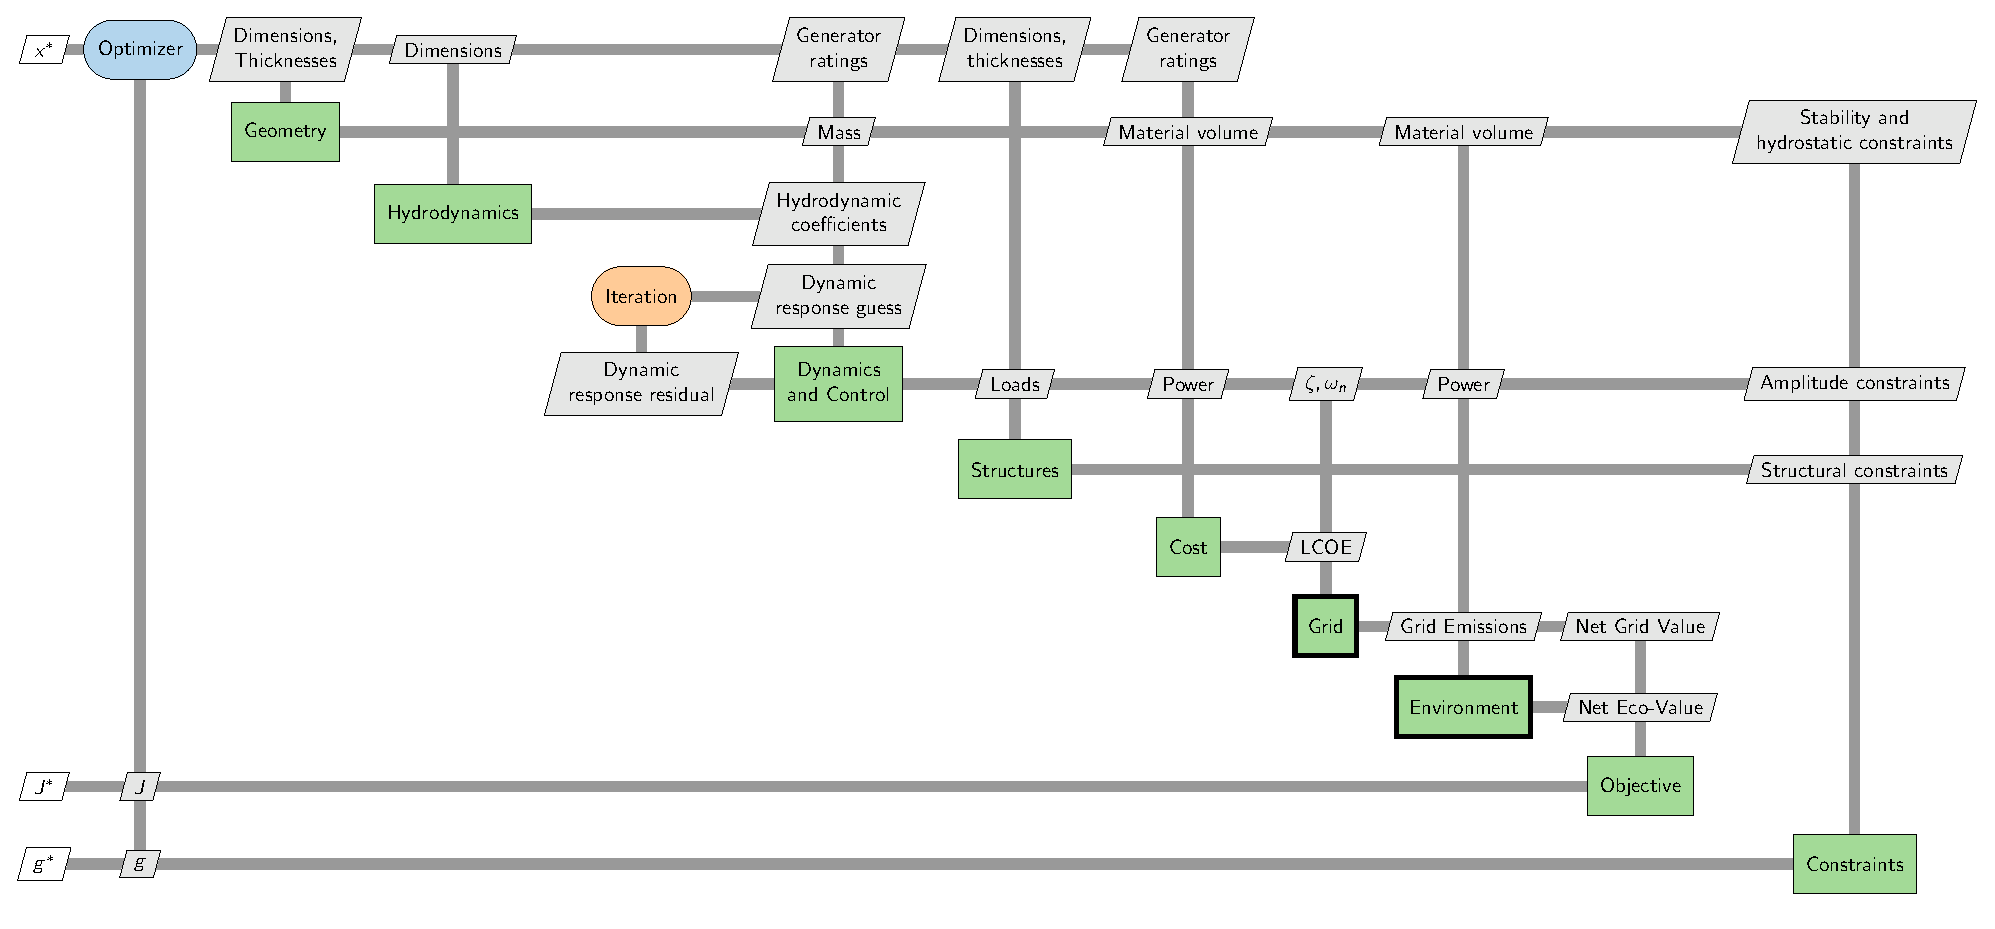
\includegraphics[width=.77\textwidth]{figures/out/xdsm_grid.pdf}
    \caption{xDSM diagram}
    \label{fig:n2}
\end{figure}
% \begin{wrapfigure}[18]{r}{0.52\textwidth}
%     \centering
%     \includegraphics[width=.5\textwidth]{figures/CEM-flowchart-idetc.png}
%     \caption{Surrogate model diagram}
%     \label{fig:surrogate}
% \end{wrapfigure}

\clearpage
\subsubsection{\textit{Capacity expansion model (CEM)}}
The GenX CEM \cite{bonaldo_genxprojectgenxjl_2025} is an open-source linear program that determines the installed capacity of each generator to minimize the total grid system cost while meeting demand and emissions constraints.
It indirectly enforces economic equilibrium since it is optimal to only install generators that cost less than the value they provide.
This implies that NVOE (net value of electricity), a metric which \cite{mowers_evaluation_2021,mccabe_system_2023} suggest, is always zero in a CEM.
The CEM grid system cost metric captures more effects than NVOE, such as costs and avoided costs of non-WEC generators, storage, and transmission required to balance the grid given the WEC power profile.
%    -  GenX: equation~\eqref{eq:CEM-objective} for the LP it solves
%\begin{equation}\label{eq:CEM-objective}
%    \min_{x_{grid}} C_{grid} = \sum_{gen} \sum_{t} p_{gen,t} x_{grid,gen,t}
%\end{equation}
    %-  time domain reduction and what timescales of power variation and demand alignment are captured vs relevant (seasonality, storms, within wave, within sea state between waves)
    %-  Emissions in CEM
    %-  how we're confident enough that the results aren't due to random chance alignment between that day's demand and wave data and are real / significant
GenX requires detailed input data on the cost, hourly profile, and existing infrastructure of all generation, transmission, storage, and load on the grid.
This is managed by the PowerGenome package \cite{schivley_powergenomepowergenome_2025}, which consolidates data from multiple sources including scenarios for reference, moderate, and high levels of electrification.
PowerGenome also allows control over a grid-wide maximum CO\textsubscript{2} constraint.
\figureautorefname~\ref{fig:CEM-data-flow} depicts the data flow for the CEM runs prior to design optimization and documents the grid data sources.
%Coefficients $\beta$ 
Grid costs and emissions are found for each input combination of WEC cost, grid scenario, location, and WEC dynamics (damping ratio and natural frequency).
Orange outlines indicate code implemented in this work rather than an existing package.
PowerGenome does not provide WEC data, so we use the MHKit interface \cite{klise_mhkit_2020} to NREL hindcast power densities \cite{wu_development_2020,allahdadi_development_2019} along with design-dependent capture width information to generate the WEC hourly power profiles. 
Temporal and spatial resolution and scope are set to hourly energy profiles for one year each decade
% for three decades, 
for a Northeast %and California 
grid scenario with three load zones.
%and two load zones respectively.
\begin{figure}[bth]
\noindent
\begin{minipage}[b]{0.64\textwidth}
    \centering
    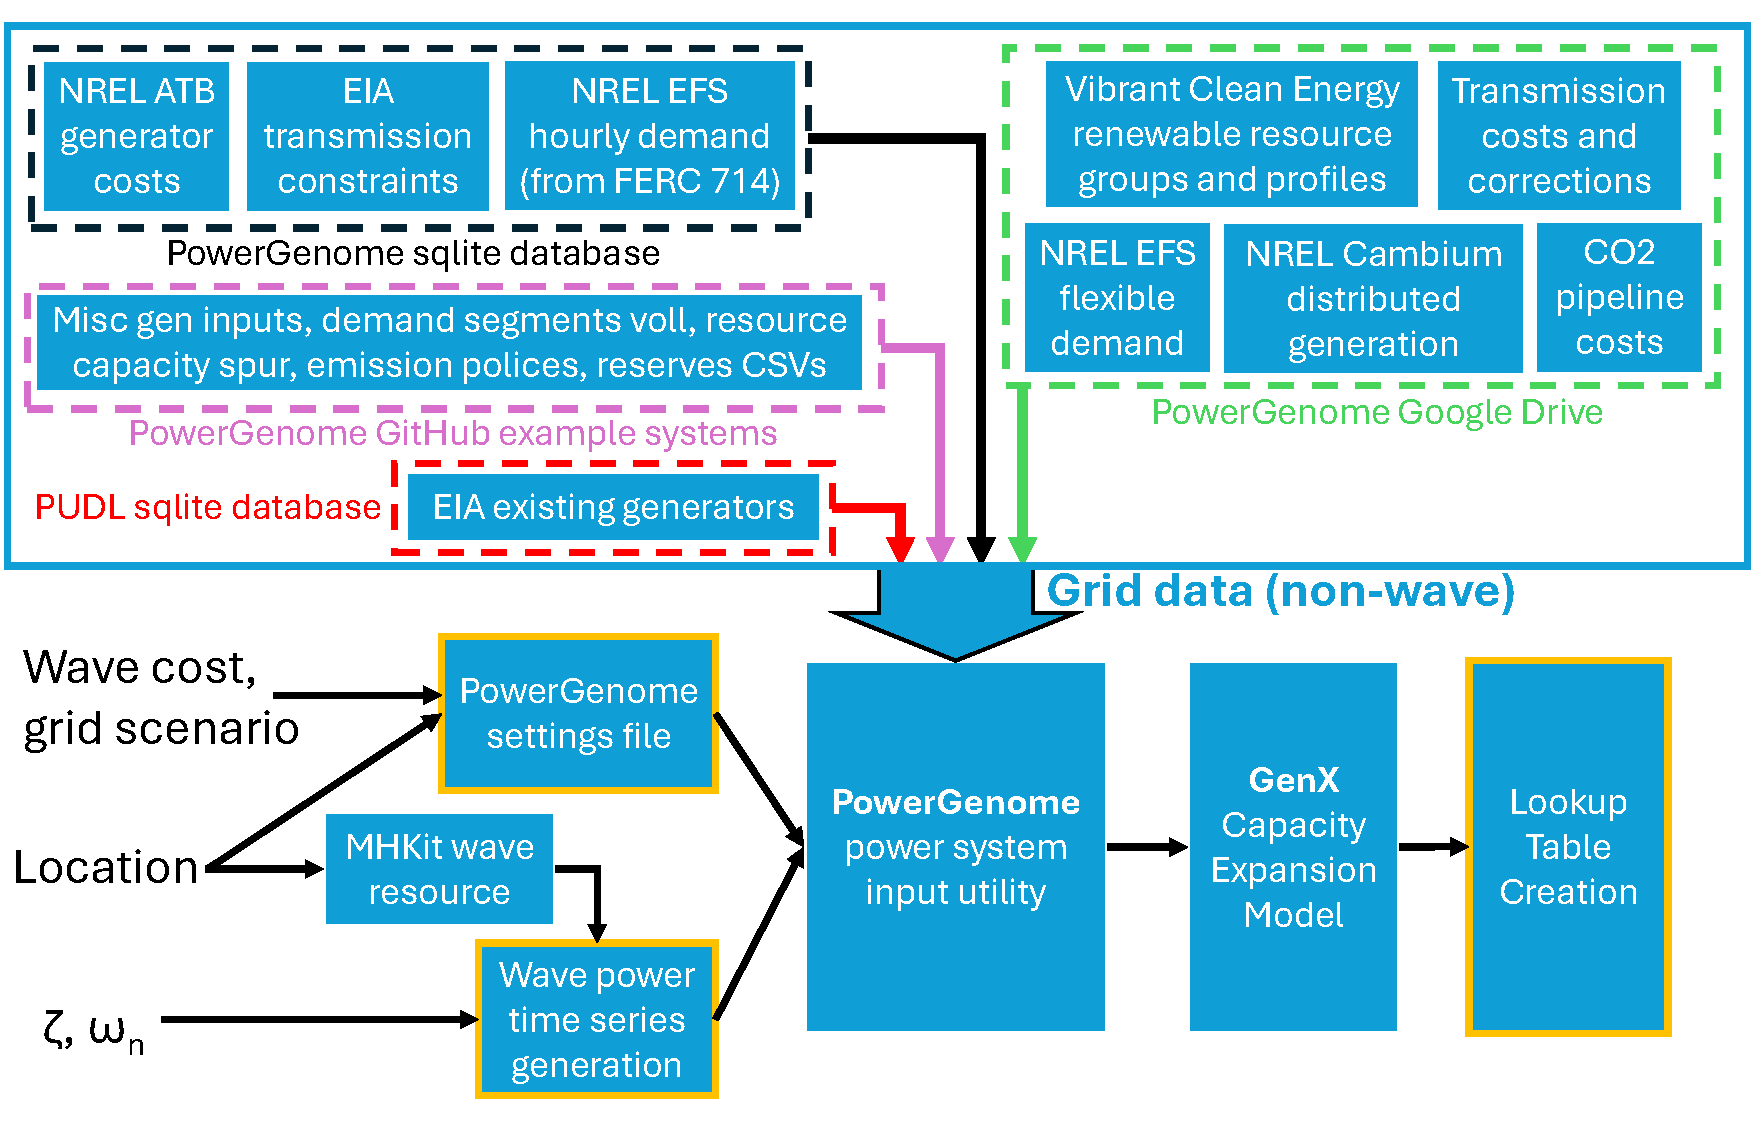
\includegraphics[width=\linewidth]{figures/PowerGenomeDataFlow_no_beta.pdf}
    \captionof{figure}{CEM data flow}
    \label{fig:CEM-data-flow}
\end{minipage}
\hfill
\begin{minipage}[b]{0.38\textwidth}
    \centering
    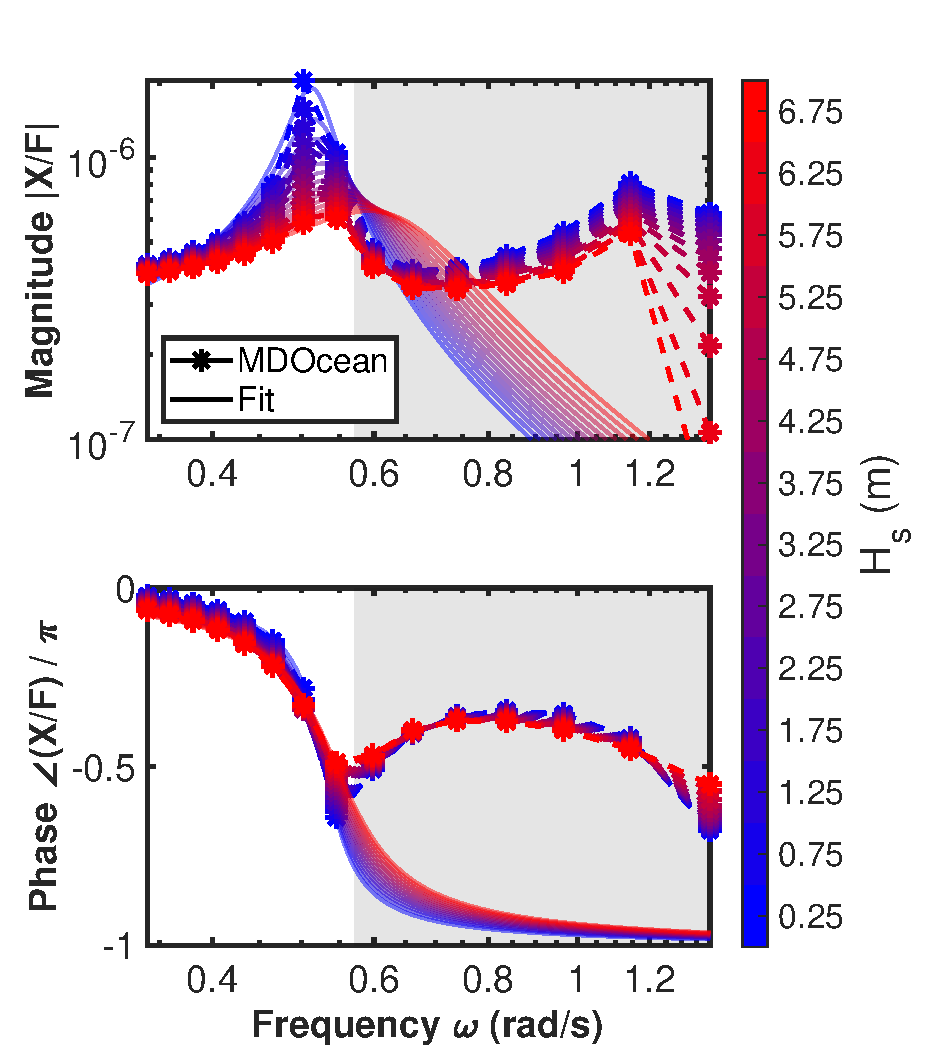
\includegraphics[width=\linewidth]{figures/bode_per_wave_height.pdf}
    \captionof{figure}{Second order Bode fit}
    \label{fig:bode}
\end{minipage}
\end{figure}
\subsubsection{\textit{Reduced order model and lookup table}}
The two WEC inputs to the CEM are capacity cost and power profile (hourly energy density times capture width $CW$ at matching wave heights and periods).
Cost can be swept easily, but $CW(H_s,T_e)$ depends on 15 additional inputs. 
A 16-dimensional sweep is computationally prohibitive, so we use a reduced order model (ROM) to collapse the WEC design space into a few key features and a surrogate model to predict CEM outputs from the reduced space.
The ROM is used only to capture the effect of WEC design on the hourly CEM variability profile, not to calculate energy.

First we nondimensionalize to reduce the design space.
The $CW(H_s,T_e)$ equation has 18 quantities: $CW$, $H_s$, $T_e$, 6 design variables, and 9 parameters.
The Buckingham-$\pi$ theorem reduces this to 15 dimensionless variables $\mathbf{\Pi_1}$ without approximation (see \appendixname~A).
To further reduce, we leverage rigid body dynamics, which dictates the following:
\begin{equation}
    \label{eq:CW-fraction}
    \frac{CW}{CW_{max}} = \frac{4 \mathcal{D}\eta_{PTO}}{G} \frac{\omega^2}{g k}  \frac{\Re(\hat{Z}_h(\mathbf{\Pi_1}))~ \Re(\hat{Z}_u(\mathbf{\Pi_1}))}{\left|\hat{Z}_h(\mathbf{\Pi_1})+\hat{Z}_u(\mathbf{\Pi_1})+\hat{Z}_d(\mathbf{\Pi_1})\right|^2}
\end{equation}
where complex impedances $\hat{Z}$ have subscript $u$ for control, $h$ for hydrodynamic radiation, and $d$ for drag.
$\mathcal{D}$ is defined in the appendix.
% response amplitude operator $\widehat{RAO}$ is the complex ratio of WEC motion to wave amplitude, $\hat{X}/\eta$.
The ROM seeks to approximate the three functions $\hat{Z}(\mathbf{\Pi_1})$ as functions of a reduced set of values $\mathbf{\Pi_2}$.
Before the design optimization, the CEM is run for all combinations of $\mathbf{\Pi_2}$.
During design optimization, we perform a least-squares fit over an error model to find the reduced groups $\mathbf{\Pi_2}$ at each iteration, and then use a surrogate model to find CEM outputs as a function of $\mathbf{\Pi_2}$. 
Currently, the surrogate model is a lookup table with linear interpolation.
Future work could develop a mechanistic surrogate model to understand CEM driving factors and allow extrapolation to different grid scenarios.

Two approaches are possible in selecting $\mathbf{\Pi_2}$ and the corresponding error model: a pole-zero description of the dynamics to obtain a low-order transfer function, or a hydrodynamics-informed curve fit.
A pole-zero description, $\mathbf{\Pi_{2,pz}}$, is easy to implement via standard system identification tools, but may require a high order to adequately capture the dynamics. 
A variety of existing WEC models use this \cite{bacelli_system_2017} or similar approaches \cite{kristiansen_state-space_2005}. 
\appendixname~A shows the equation for an arbitrary number of poles and zeros.
Alternatively, a custom hydrodynamics curve fit, $\mathbf{\Pi_{2,hyd}}$, offers more accuracy at lower order using deep mechanistic understanding of the physics. \appendixname~A shows a fit to describe radiation impedance $\hat{Z}_h$ as a function of $kh$ using only two parameters.

This study evaluates a second-order pole-zero model $\mathbf{\Pi_{2,pz}=(\zeta,\omega_n)}$ to fit the closed loop system compliance, $\hat{X}/\hat{F}=1/(i\omega(\hat{Z}_h+\hat{Z}_u+\hat{Z}_d))$,  but finds a poor fit.
Specifically, \figureautorefname~\ref{fig:bode} shows that for the nominal RM3, the model is valid only at frequencies at and below resonance.
Capturing behavior above resonance would require a higher order model such as one with five poles, two standard zeros, and two right half plane zeros to capture the abrupt increase in phase.
This is similar to another study where a point absorber intrinsic impedance $\hat{Z}_h + \hat{Z}_d$ was fit with three poles and one right half plane zero \cite{bacelli_system_2017}.
However, sweeping this many dynamic inputs to the CEM is impractical, and high frequencies are less common in the ocean, so here we maintain a second order model and exclude frequencies with $\omega>0.6$ from the fit (shown in grey).
Fitting each wave height separately lets the model capture drag nonlinearities, which manifest as a roughly locally linear dependence of $\zeta$ and $\omega_n$ on wave height.
\figureautorefname~\ref{fig:fit-versus-wave-height} shows this relation when fitting magnitude and phase separately.
The magnitude fit depends significantly more on $H_s$ than the phase fit.
Mismatch of magnitude and phase fits at low $H_s$ is evidence of a nonminimum phase system, and the larger mismatch at high $H_s$ is due to drag nonlinearities.
While it doesn't affect the shape of $\hat{Z}(\omega)$, stiffness $K$ also shows nonlinearity.

Difficulty capturing high-frequency behavior is expected from the model structure. 
A second-order system has equivalent damping $B=\Re(\hat{F}/(i\omega\hat{X}))=2\zeta/\omega_n$, which is constant across frequency, and equivalent reactance $K-(m+A)/\omega^2=\Re(\hat{F}/\hat{X})\sim 1-\omega^2/\omega_n^2$, which only permits added mass frequency-dependence of the form $A = A_\infty + A_0/\omega^2$ \cite{franklin2014feedback}.
This does not align with the true shape of $\hat{Z}_h(\omega)$, in which $B$ decreases (perhaps after an initial increase) and $A$ often has local minima and maxima.
Future work should better explore hydrodynamic curve fits $\mathbf{\Pi_{2,hyd}}$.
%Combined with the impedance relation $\hat{Z}=1/\widehat{RAO} \cdot \hat{F}/\eta$ for excitation force $\hat{F}$, and the optimal reactive control law $B_u(\omega) = \Im(\hat{Z}(\omega))/(2\omega)$, this forces a form for the control damping related to $\hat{F}/\eta$ the excitation coefficient.



%In addition to the directly used CEM outputs of grid cost and emissions, we use additional CEM outputs (installed capacity of WECs and other generators) and compute indirect CEM outputs (maximum cost threshold) as part of the surrogate model to predict the primary outputs from design inputs. 
%The maximum threshold cost represents the maximum cost of any generator (with the most favorable generation profile) that would be installed for each grid scenario.
\begin{figure}[bth]
\noindent
\begin{minipage}[b]{0.565\textwidth}
    \centering
    %\placeholdertrue
    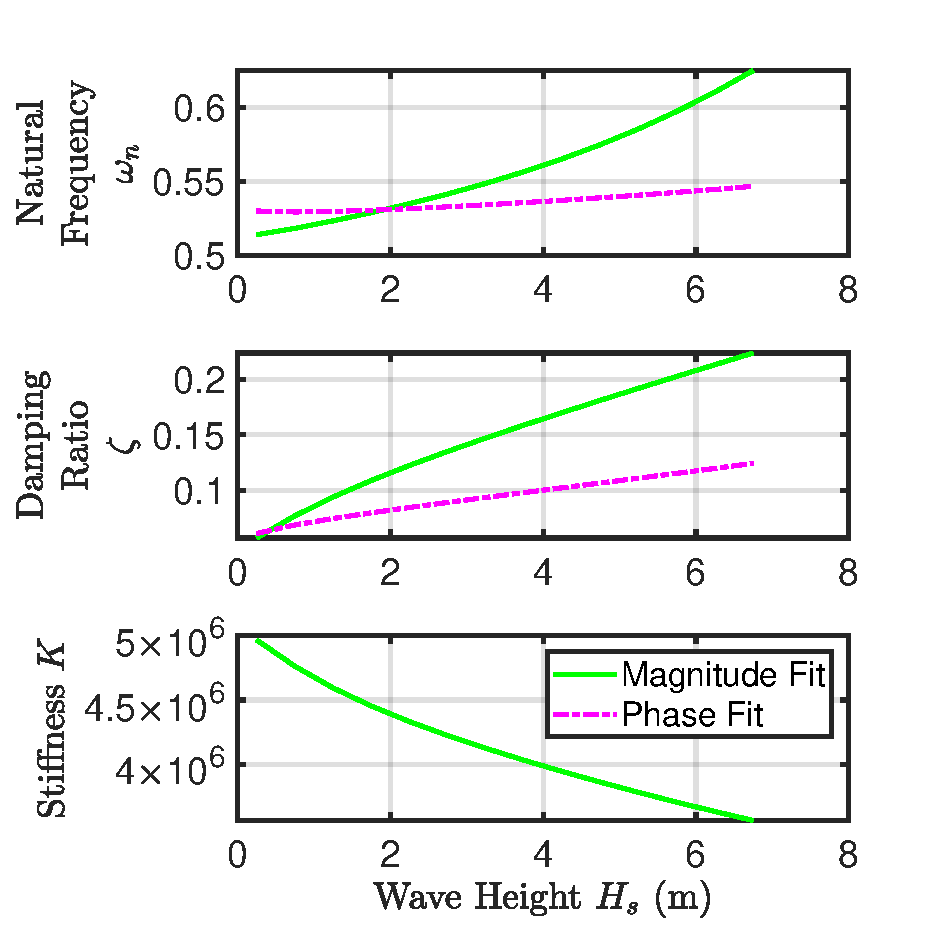
\includegraphics[width=\linewidth]{figures/fit_wave_height_trend.pdf}
    \captionof{figure}{Variation of fit parameters with wave height}
    \label{fig:fit-versus-wave-height}
\end{minipage}
\hfill
\begin{minipage}[b]{0.435\textwidth}
    \centering
    %\placeholdertrue
    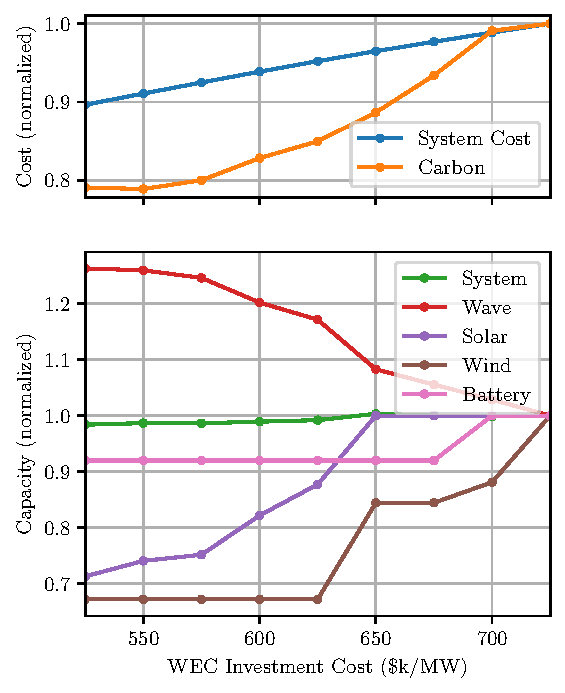
\includegraphics[width=\linewidth]{figures/CEM_cost_sweep.pdf}
    \captionof{figure}{CEM cost sweep for ISONE}
    \label{fig:cem-cost-sweep}
\end{minipage}
\end{figure}

%In optimal reactive control, $B_u(\omega)=B_h(\omega)+B_d(\omega,RAO(\omega))$, where $B_h$ is the hydrodynamic damping and $B_d$ is nonlinear drag damping.
%We assume the closed-loop RAO is a standard second order system with damping ratio $\zeta$ and natural frequency $\omega_n$.
%The values of $\zeta$ and $\omega_n$ for a given design are determined via a least-squares fit of the dynamics module output for $\hat{X}$ to the second order form.% across all sea states with nonzero probability in the JPD.
%Using imaginary unit $i$, wave height index $j$, and frequency index $k$, this is expressed:
%(equation~\eqref{eq:bode-fit}),
%\begin{equation}
%\begin{aligned}
%    \zeta,\omega_n &= \mathrm{argmin}\left( \epsilon_{mag}^2 + \epsilon_{phase}^2 \right) \\
%    \epsilon_{mag} &= xxx \\
%    \epsilon_{phase} &= xxx
%\end{aligned}
%\end{equation}
% \begin{equation}\label{eq:bode-fit}
%     \zeta,\omega_n = \mathrm{argmin}(\epsilon_{mag}^2)
%     ,\quad
%     \epsilon_{mag} = \sum_{j,k}^{} \left(\left|\frac{\hat{X}_{jk}}{\eta_j}\right|-\left|\widehat{RAO}(\omega_k)\right|\right)
%     ,\quad
%     \widehat{RAO}(\omega) = \frac{1}{1-\left(\frac{\omega}{\omega_n}\right)^2 + i 2 \zeta \frac{\omega}{\omega_n}}
% \end{equation}

% It is also required to model 
% \begin{equation}
%     B_u = \overline{B_{u}} \omega \exp(-\omega^2)
% \end{equation}
    %- assumes that the WEC can generate less than its max power without violating any amplitude/force constraints        
    %-  how CEM system cost gets turned into NVOE metric (since CEM enforces NVOE=0)    
\subsubsection{\textit{Life cycle analysis (LCA)}}
LCA in the early design phase is challenging due to uncertainties in materials, manufacturing, and transportation \cite{moni_life_2020}.
Fortunately, optimization only requires modeling effects that meaningfully scale with design variables.
This includes material use (steel, fiberglass) but not aquatic habitat disruption or hydraulic fluid toxicity since they are not captured in MDOcean's low design fidelity.
Although the present study holds distance from shore constant, the environmental model includes offshore transportation (diesel fuel) so future work can evaluate the tradeoff between better energetics but worse survivability, operating cost, and maintenance emissions for WECs further offshore.

MDOcean's geometry module calculates WEC material masses and the environment module multiplies by appropriate weighting coefficients from the Idemat LCA dataset \cite{van_den_herik_idemat_2024}. These are scope 3 eco-cost coefficients \cite{vogtlander_lca-based_2010} that express diverse lifetime environmental impacts (i.e. water, emissions, pollution) of various materials and processes in monetary units (see \tableautorefname~\ref{tab:lca-weights}).
We convert Euros to USD via the March 2024 exchange rate of 1.09 \$/\texteuro.
MDOcean then offsets the eco-cost with the eco-value of CEM avoided grid emissions using the social cost of carbon. Finally, it normalizes by CEM WEC grid energy production to obtain the net eco-value per unit energy (\$/kWh).
\begin{minipage}[m]{0.34\textwidth}
    \begin{table}[H]
    \begin{tabular}{ ll } 
        \hline
        Component & Value \\ 
        \hline
        Steel & 0.192 \$/kg \\ 
        Fiberglass & 6.950 \$/m\textsuperscript{2} \\ 
        Dist. from shore & 65.88 \$/mile \\ 
        Social cost of CO\textsubscript{2} & 0.145 \$/kgCO\textsubscript{2} \\
    \end{tabular}
    \caption{Eco-cost coefficients}
    \label{tab:lca-weights}
    \end{table}
\end{minipage}
\hfill
\begin{minipage}[m]{0.65\textwidth}
    \vspace{.2\baselineskip}
    \setlength{\parindent}{1.5em}
    The nominal RM3
    %, which uses 667 tonnes of steel, has a hull area of 924 m\textsuperscript{2}, and is 3.4 miles from shore, 
    eco-cost is \$134,800 per WEC.
    95\% is from steel, 5\% from fiberglass, and <1\% from transportation.
    Using the social cost of carbon, each WEC must displace >930 tonnes of CO\textsubscript{2} emissions on the grid over its lifetime to ``break even" (achieve a net positive eco-value).
    With an annual energy production of 500 MWh and 20 year lifetime, it must displace 0.093 tonnes of CO\textsubscript{2} per MWh.
    Typical natural gas and coal plants emit around 0.5 and 1.0 tonnes of CO\textsubscript{2} per MWh respectively.
    Therefore, for each MWh of energy that RM3 generates, it must displace at least 0.18 MWh of natural gas or 0.09 MWh of coal to have a positive net eco-value.
%     Inspecting the model reveals two takeaways.
%     First, the eco-cost computed here represents only \hl{XX}\% of the eco-cost of prior WEC LCA studies \cite{pennock_life_2022}, indicating that most of the eco-cost \hl{(is/is not)} cemented \hl{(before/until)} the detail design phase.
%     First, the eco-value far exceeds the eco-cost, meaning LCA-informed environmental optimization to reduce WEC eco-cost is less relevant than economic optimization to help WECs displace fossil fuels.
%     Second, eco-cost coefficients for steel and fiberglass are similar to their economic prices, so the least-cost and least-eco-cost designs should be similar.
%     % show this with numbers
%     Both of these observations imply that design-for-environment techniques have limited utility at the early design stage, although multi-objective optimization is still performed to confirm this conclusion.
\end{minipage}
\vspace{-\baselineskip}
\section{Results and conclusions}
It took 20 minutes to run the 15 CEM optimizations on an Ubuntu 20.04 server with Intel(R) Core(TM) i9-10940X CPU @ 3.30GHz, using up to 28 threads for each optimization and executing successive optimizations in series. Of this time, only around half is spent in GenX, since PowerGenome takes 35 seconds per case. %, downloading MHKit data takes 17 seconds, 
%It took \hl{XX} minutes to run the design optimization, with each simulation taking \hl{XX} ms and each single-objective optimization taking \hl{XX} iterations.
Figure~\ref{fig:cem-cost-sweep} shows the normalized grid cost, CO2 emissions, and capacity from the CEM for a WEC with $\zeta=0.05, \omega_n=0.4$, and $B_{u}=10^5\omega e^{-\omega^2}$ (a Rayleigh distribution: an alternative model to the one in \appendixname~A) in the Northeast.
%These results have WEC capacities of zero in the yellow regions due to a lack of economic viability, and therefore have constant system cost and emissions there.
As the WEC gets cheaper (moving from right to left), %and more consistent power profile,
the grid cost, emissions, and capacity of other renewables reduce as expected, and WEC capacity increases.
Capacity behaves nonlinearly: cheaper WECs first displace wind, then batteries, then solar.
The different ``cut-in costs'' to displace each technology likely reflect both capital costs and power profiles.
The x-axis width of the cut-in reflects the heterogeneity of each resource. For example, the batteries displaced are very homogeneous, with all sites having a cut-in cost of 675-700 \$k/MW, but wind and solar have a wide range of cut-in costs due to resource variation across sites.
Unlike capacity, system cost varies linearly with WEC cost.
The slope has a useful sensitivity interpretation: for every $30\%$ WEC cost reduces, system cost reduces $10\%$.
Meanwhile, emission reduction is moderately linear with WEC cost, but appears more strongly linear with WEC capacity.
The most expensive designs have a ratio of fossil fuel energy displaced to WEC energy produced of 0.075, below the 0.09-0.18 requirement.
Even if RM3 was economically viable, it does not avoid enough emissions to be environmentally viable. This shows the importance of both economic and environmental considerations in design optimization.
%For both $\zeta$ and $\omega_n$, we expect to see local optimum behavior, \hl{where} $\zeta=XX$ and $\omega_n=XX$ are the best values from the perspective of hourly variability, and values above and below are less optimal.
%The most optimistic combination of $\zeta$ and $\omega_n$ tested (not necessarily achievable while obeying design constraints), reduce the grid cost by around \hl{XX}\%.
%The effect on emissions is more pronounced, with the most optimistic combination reducing emissions by around \hl{XX}\%.
%This lets us draw the overall conclusion that \hl{XX}.

Further examination of the time-series results is required to understand if WECs in this system primarily derive value from seasonal balancing, consistency, availability at peak times, or some other characteristic.
Additionally, sweeping all design parameters and grid scenarios remains necessary to populate the lookup table for design optimization, and to more broadly understand the grid value of WECs' unique temporal power profile and its dependence on design.
Future work could examine the sensitivity of CEM results to the resource and demand data year to avoid overfitting, especially since wave resource data is not aggregated across sites as PowerGenome does for wind and solar.
Finally, design optimization results will yield insight into whether and how the objective values and optimal design features meaningfully vary when optimizing for LCOE, grid cost, or net eco-value across various grid scenarios.
%-  can the CEM results be predicted by correlation coefficient of WEC power with demand or with energy storage or with lost load of solar, the capacity factor, sum of hourly profit, other proxies?

% Proceeding to the design optimization results, \figureautorefname~\ref{fig:single-obj-compare} visualizes the optimal designs for the various objectives, alongside the standard RM3 for reference.
% The WEC optimized for grid cost is \hl{(larger/smaller)} compared to the one optimized for LCOE.
% Meanwhile, the WEC optimized for the net eco-value per energy is (the same as, with \hl{XX} exceptions) the one optimized for grid cost.
% \figureautorefname~\ref{fig:pareto} shows the Pareto front of the multi-objective optimization.
% We observe \hl{XX} about the tradeoff, which \hl{(confirms/negates)} the suggestion from the environmental model inspection that the two objectives minimally conflict.
% While this study initially hypothesized a meaningful environmental-economic tradeoff, insights obtained by building the model suggests that economic and environmental objectives align in the early design phase.
% This means that environmentally-conscious engineers and policymakers can feel satisfied that here, economic optimization also directly benefits the environmental bottom line.
% \figureautorefname~\ref{fig:design-heuristics} shows the design heuristics for the pareto front.
% As we transition from economically optimal WECs to environmentally optimal WECs, the bulk dimensions \hl{(grow/shrink)}, the generator ratings \hl{(grow/shrink)}, and the structural thicknesses \hl{(grow/shrink)}.


% \begin{figure}[t]
% \noindent
% \begin{minipage}[t]{0.325\textwidth}
%     \centering
%     \placeholdertrue
%     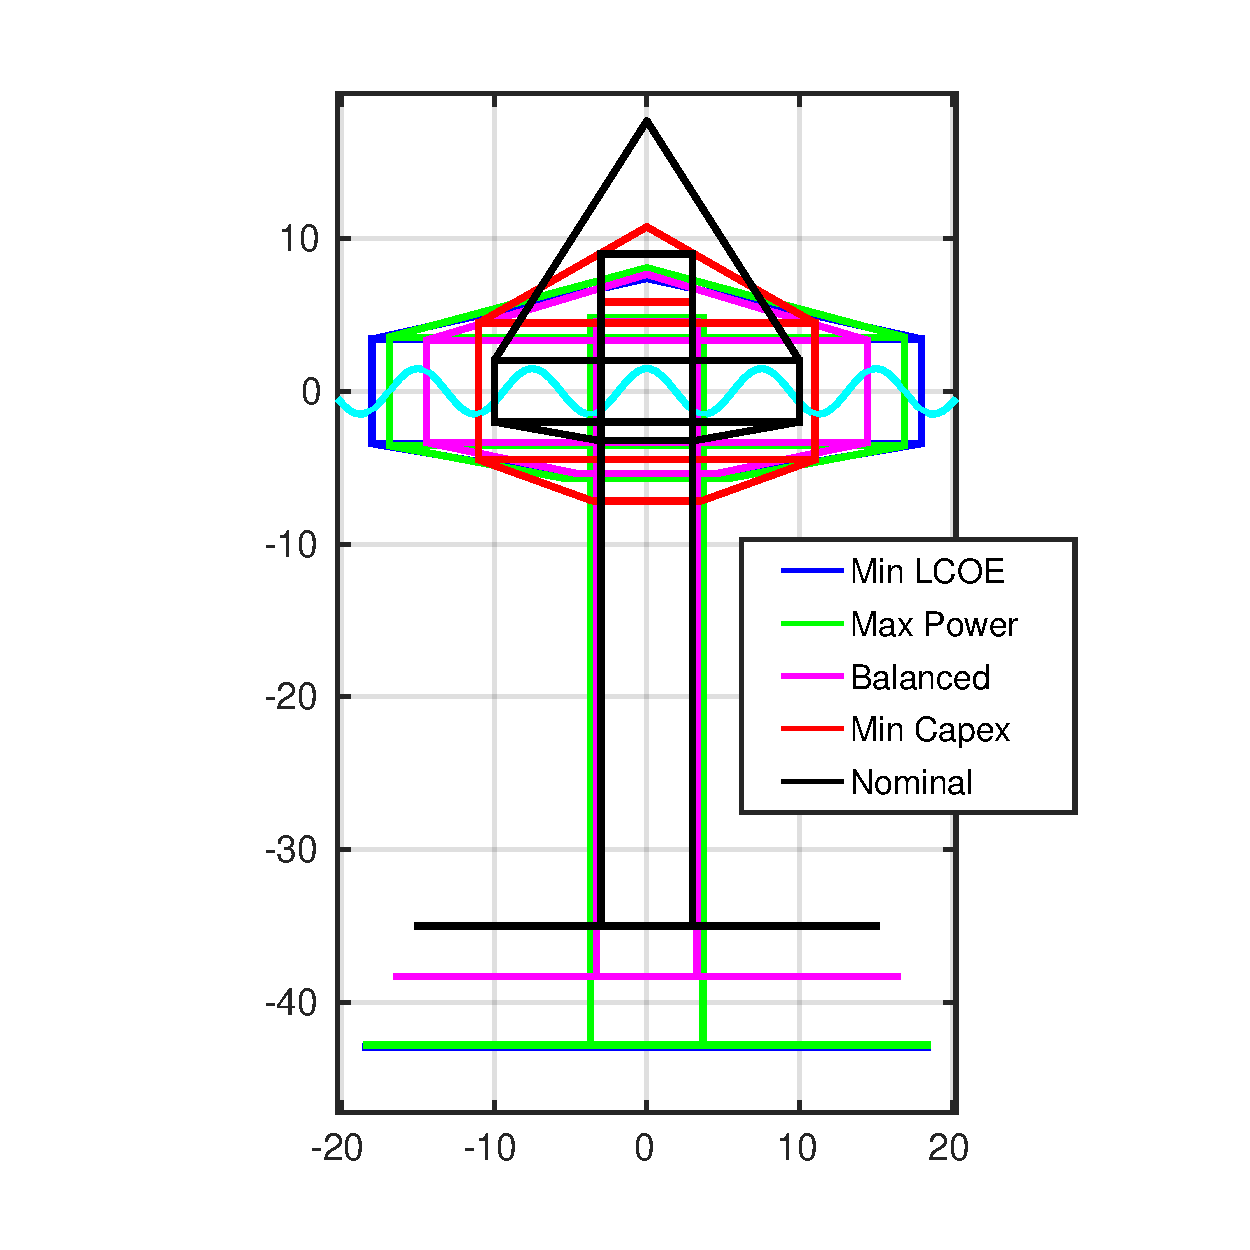
\includegraphics[width=\linewidth]{figures/mdocean_geometry_compare.pdf}
%     \captionof{figure}{Single-objective optima}
%     \label{fig:single-obj-compare}
% \end{minipage}
% \hfill
% \begin{minipage}[t]{0.325\textwidth}
%     \centering
%     \placeholdertrue
%     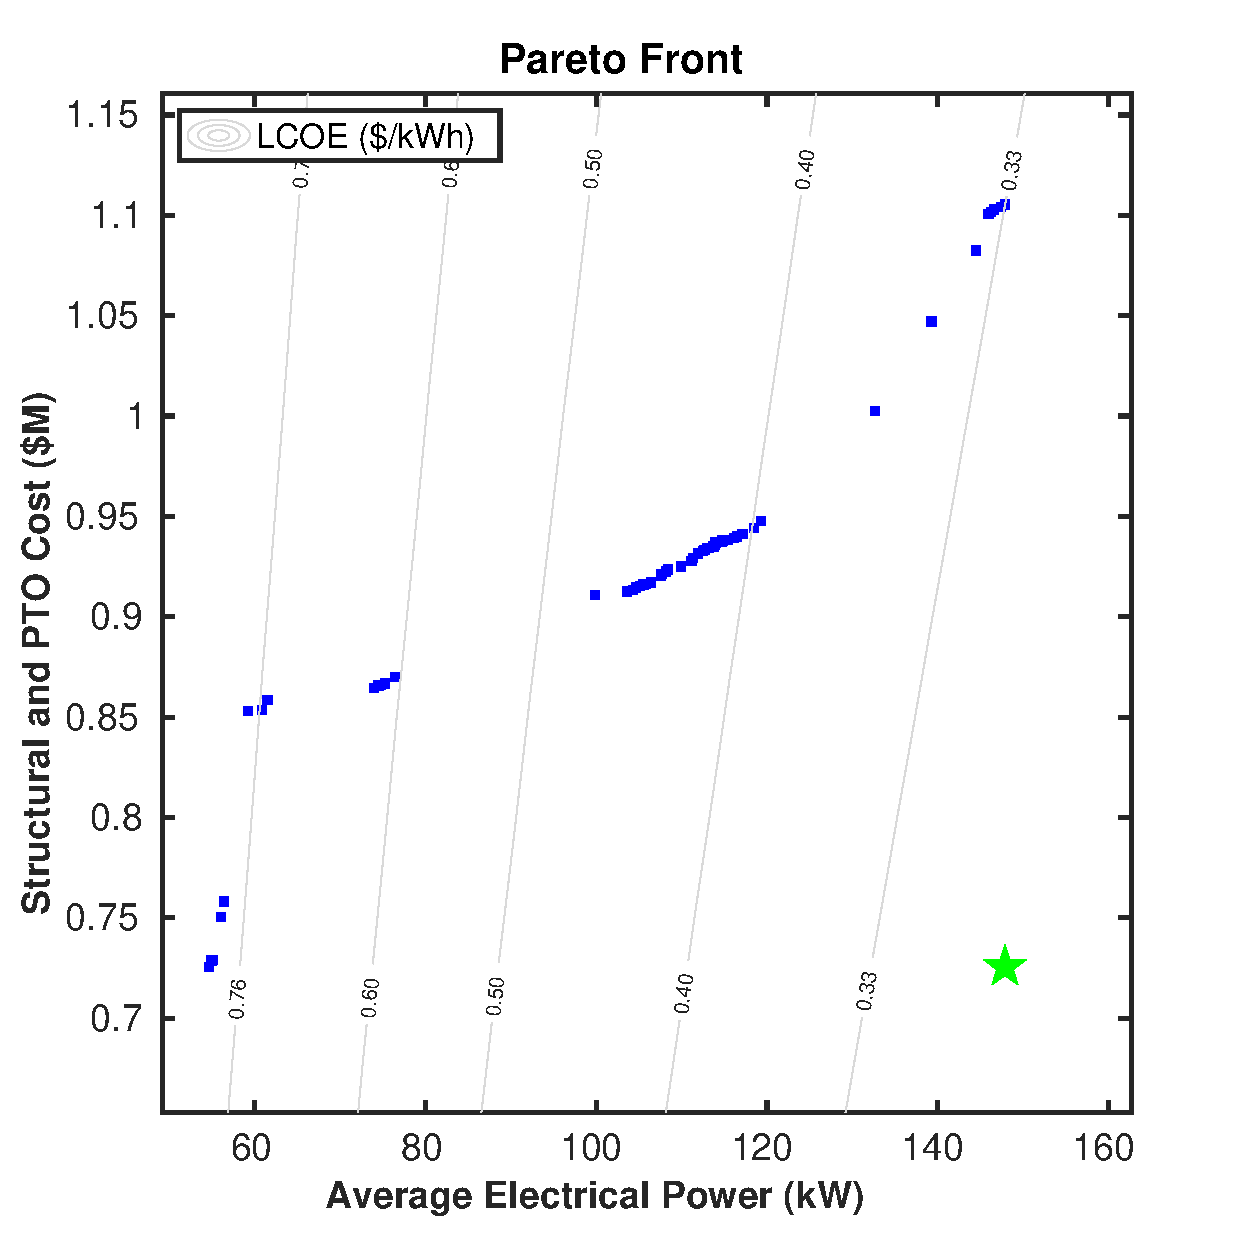
\includegraphics[width=\linewidth]{figures/mdocean_pareto.pdf}
%     \captionof{figure}{Pareto front}
%     \label{fig:pareto}
% \end{minipage}
% \hfill
% \begin{minipage}[t]{0.3\textwidth}
%     \centering
%     \placeholdertrue
%     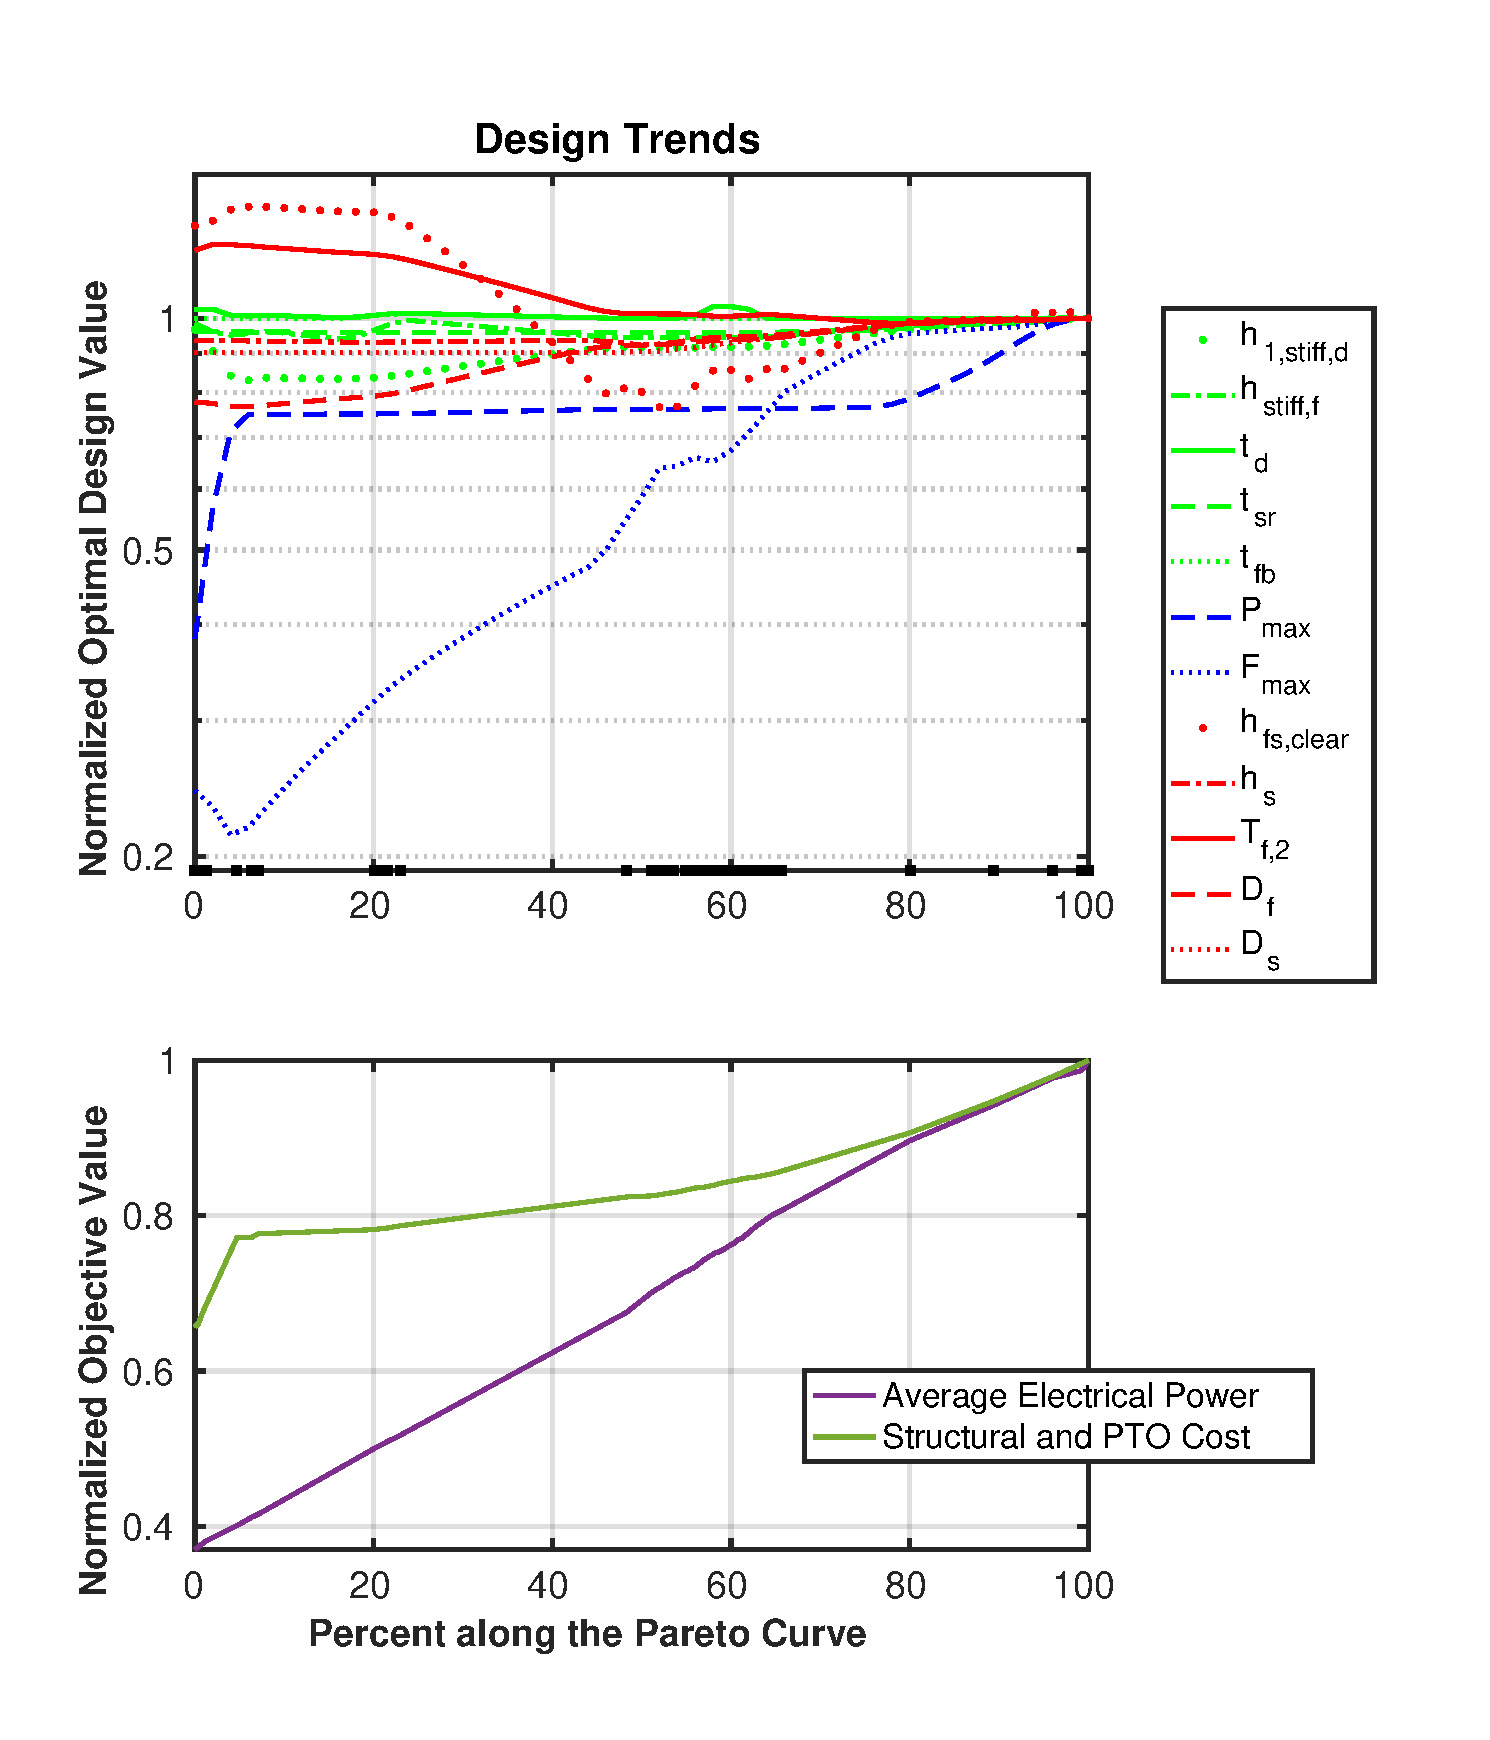
\includegraphics[width=\linewidth]{figures/mdocean_design_heuristics.pdf}
%     \captionof{figure}{Design heuristics}
%     \label{fig:design-heuristics}
% \end{minipage}
% \end{figure}

% \section{Conclusions}
% When assessed in a CEM that accounts for their temporal value, WECs are actually quite close to viable, despite a high LCOE.
% We also find that optimizing for grid system cost instead of LCOE makes a big difference in the optimal design.
% \hl{XX}. 

\section*{Acknowledgments and Data Availability}
%%%%%%%%%%%%%%%%%%%%%%%%%%%%%%%%%%%%%%%%%%%%%%%%%%%%%%%%%%%%%%%%%%%%%%%%%%%%%%%%%%%%%%%%%%%%%%%%%%%%%%%%
We thank Olivia Vitale and Collin Treacy for feedback on a draft. Open-source code: design optimization at \url{github.com/symbiotic-engineering/MDOcean} and CEM at \url{github.com/symbiotic-engineering/wec-decider}.

\clearpage

% \begin{framed}
% \textbf{Nomenclature} \\
% \normalsize    
%     A\ \ \ \ radius of \\    
%     B \ \ \ \ position of \\    
%     C\ \ \ \ further nomenclature continues down the page inside the text box \\
% \end{framed}

% Headings should be placed above tables, left justified.

% The figure number and caption should be typed below the illustration in 8 pt.

%%%%%%%%%%%%%%%%%%%%%%%%%%%%%%%%%%%%%%%%%%%%%%%%%%%%%%%%%%%%%%%%%%%%%%%%%%%%%%%%%%%%%%%%%%%%%%%%%%%%%%%%
\section*{Appendix A. Reduced order model details}
The $CW(H_s,T_e)$ equation initially involves 18 quantities: $CW$, $H_s$, $T_e$,
6 design variables (generator ratings $F_{lim}$ and $P_{lim}$ and float and spar diameters $D_f$ and $D_s$ and drafts $T_f$ and $T_s$), 
and 9 parameters (damping plate diameter and thickness $D_d$ and $h_d$, efficiency $\eta_{PTO}$, float and spar drag coefficient $C_{d,f}$ and $C_{d,s}$, damping versus reactive control type $C$, water depth $h$, water density $\rho$, and acceleration of gravity $g$). 
These span three physical dimensions (length, time, and mass).
By the Buckingham-$\pi$ theorem, the relationship can be reduced to a function of $18-3=15$ dimensionless groups \cite{mckinley_dimensional_2021}. 
Capture width is nondimensionalized by the maximum radiative capture width, $CW_{max}=Gg/\omega^2$, with gain $G$ (1 for heave, 2 for surge/pitch) and frequency $\omega$ \cite{zou_practical_2023}. % 1 
Wave height is divided by water depth. % 2
Wave period is captured as the product of wavenumber and water depth, $kh$. % 3
Generator force and power limits are nondimensionalized by the force and power at the maximum capture width, $F_{max}$ and $P_{max}$. % 4-5
The six dimensions are divided by each other or the water depth.% 6-11
The efficiency, drag coefficients, and control type are already nondimensional. % 12-15
Thus, we have the following $\mathbf{\Pi_1}$ dimensionless groups:
\begin{equation}
    \frac{CW}{CW_{max}} = f\left( \mathbf{\Pi_1} \right) = f\left(\frac{H_s}{h}, kh, 
    \frac{P_{lim}}{P_{max}}, \frac{F_{lim}}{F_{max}},
    \frac{D_f}{h}, \frac{D_s}{D_f}, \frac{T_f}{T_s}, \frac{T_s}{h}, \frac{D_d}{D_f}, \frac{t_d}{D_d}, 
    \eta_{PTO}, C_{d,f}, C_{d,s},  C\right)
\end{equation}
Moving to the pole-zero ROM, a general model with $C_P$ complex pole pairs, $C_Z$ complex zero pairs, $R_P$ real poles, and $R_Z$ real zeros has a total of $2C_P+2C_Z+R_P+R_Z$ parameters and is expressed as:
\begin{equation}
    \mathbf{\Pi_{2,pz}} =  \left(
        \zeta_{p},~ \omega_{n,p},~
        \zeta_{z},~ \omega_{n,z},~
        \tau_{p},~ 
        \tau_{z} 
        \right),
    \quad
    \frac{\hat{X}}{\hat{F}} = 
    \prod_{r_p=1}^{R_P} 
    \prod_{r_z=1}^{R_Z} 
    \prod_{c_p=1}^{C_P}
    \prod_{c_z=1}^{C_Z}
    \frac{1+\tau_{z,r_z} i \omega}
         {1+\tau_{p,r_p} i \omega}  \times
    \frac{1-\left(\frac{\omega}{\omega_{n,c_z}}\right)^2 + i 2 \zeta_{c_z} \frac{\omega}{\omega_{n,c_z}}}
         {1-\left(\frac{\omega}{\omega_{n,c_p}}\right)^2 + i 2 \zeta_{c_p} \frac{\omega}{\omega_{n,c_p}}}
    \quad
\end{equation}
The pole-zero ROM tested in the paper uses $C_P=1, C_Z=R_P=R_Z=0$.

Alternatively, the following custom hydrodynamics curve fits radiation impedance as a function of $kh$ using only two parameters, $kD_f$ and $B_0^e$. The latter is approximated as constant, neglecting frequency and geometry dependence:
\begin{equation}\label{eq:hydro-fit}
    \mathbf{\Pi_{2,hyd}} = (kh, kD_f, B_0^e),
    \quad
    \frac{\hat{F}}{\eta} = \frac{-4i\rho g h \sqrt{N_0}B_0^e}{\cosh(kh)~H_0(kD_f/2)},
    \quad
    B_h = \frac{k \omega~ |\hat{F}/\eta|^2}{2 \mathcal{D} \rho g^2},
    \quad
    A = \frac{1}{\pi \omega} \displaystyle \operatorname {p.\!v.}\int_0^\infty \frac{B(t)}{t-kD_f/2} dt
\end{equation}
The $\hat{F}/\eta$ equation leverages the eigenfunction form of the excitation coefficient for axisymmetric bodies, where $H_0$ is the Hankel function and $N_0=\frac{1}{2}\left(1+\frac{\sinh(2kh)}{2kh}  \right)$ \cite{chau_inertia_2012}.
The $B_h$ equation applies the Haskind relation to obtain the damping, where $\mathcal{D}=\tanh(kh)+kh(1-\tanh^2(kh))$ \cite{chau_inertia_2012}.
The $A$ equation applies the Kramers-Kronig relation to obtain the added mass, where $\operatorname {p.\!v.}$ is Cauchy principal value \cite{greenhow_added_1988}.
Note that \eqref{eq:hydro-fit} only yields a fit for $\hat{Z}_h$ and does not attempt to capture the effect of drag nonlinearities ($\hat{Z}_d$) or impedance mismatch due to force limit, power limit, or damping control ($\hat{Z}_u$), although it is expected that mechanistic curve fits for these effects could be developed using only 2-3 additional parameters, as opposed to the 5 such groups in $\mathbf{\Pi_1}$.
% %%%%%%%%%%%%%%%%%%%%%%%%%%%%%%%%%%%%%%%%%%%%%%%%%%%%%%%%%%%%%%%%%%%%%%%%%%%%%%%%%%%%%%%%%%%%%%%%%%%%%%%%
% $C$ refers to costs (\$M) (output from CEM), $S$ refers to specific capacity costs (\$M/kW) (input to CEM), $x_{grid}$ refers to installed capacities (decision variable in CEM), and $E$ refers to specific energy costs (\$/kWh). The amount of built wave capacity $x_{grid,WEC}$ is not to be confused with $x_{design}$, the WEC design variables in the outer (MDOcean) optimization that are parameters (held constant) in the CEM.

% \begin{equation}
% \begin{aligned}
%     C_{grid}(p_{grid},x_{design}) &= C_{grid,0}(p_{grid})- \beta_1(p_{grid})~ x_{grid,WEC}(p_{grid},x_{design}) \\
%     \frac{x_{grid,WEC}(p_{grid},x_{design})}{x_{grid,WEC}(p_{grid},x_{design})+\sum_{gen\neq WEC}x_{grid,gen}(p_{grid},x_{design})} &= \min\left(\beta_2(p_{grid}) \times \max\left(\frac{S_{WEC,thresh}(p_{grid},x_{design})}{S_{WEC}(x_{design})}-1,0\right), 1\right) \\
%     S_{WEC,thresh}(p_{grid},x_{design}) &= S_{max,thresh}(p_{grid}) - \beta_3(p_{grid}) \zeta(x_{design}) - \beta_4(p_{grid}) \frac{\omega_n}{\omega_p}(x_{design}) - \beta_5(p_{grid}) \min\left(\frac{P_{max}}{P_{pk}}(x_{design}),1\right) \\
%     \sum_{gen\neq WEC}x_{grid,gen}(p_{grid},x_{design}) &= \sum_{gen}x_{grid,gen,0}(p_{grid})-\beta_6(p_{grid}) \zeta(x_{design}) - \beta_7(p_{grid}) \frac{\omega_n}{\omega_p}(x_{design}) - \beta_8(p_{grid}) \min\left(\frac{P_{max}}{P_{pk}}(x_{design}),1\right)
% \end{aligned}
% \end{equation}

%improvements to make to above eqn:
%- debatable whether coeffs should be kept dimensional, ie should $\beta_1$ get divided by total capacity and $C_{grid,0}(p_{grid})$ so it's relating percent cost to percent capacity?
%- $\beta_{3-8}$ terms could be made nonlinear as needed - ie $(\frac{\omega_n}{\omega_p})^2-1$ shows up in theory. I could also try to feed-forward incorporate the time domain power reconstruction, ie a peak to average ratio, if that is looking like a better fit than the freq domain stuff, but that just tells me that my hope of doing freq domain to connect to mdocean won't work out.
%- ideally some of these betas turn out to be independent of p grid, which means more of the p grid dependence can be found just from the 0 (no wec) case for that p, without requiring a whole design sweep. That is the reason all this modeling is potentially more useful than a lookup table.
%- Could add saturation to make sure $S_{WEC,thresh}>0$ and $C_{grid}>0$.
%- add hats or some other notation to differentiate predicted (fit) from actual

\printbibliography

\end{document}